
\documentclass[a4paper, oneside, 11pt]{report}
\usepackage{epsfig,pifont,float,multirow,amsmath,amssymb}
\newcommand{\mc}{\multicolumn{1}{c|}}
\newcommand{\mb}{\mathbf}
\newcommand{\mi}{\mathit}
\newcommand{\oa}{\overrightarrow}
\newcommand{\bs}{\boldsymbol}
\newcommand{\ra}{\rightarrow}
\newcommand{\la}{\leftarrow}
\usepackage{algorithm}
\usepackage{algorithmic}
\topmargin = 0pt
\voffset = -80pt
\oddsidemargin = 15pt
\textwidth = 425pt
\textheight = 750pt

\begin{document}

\begin{titlepage}
\begin{center}
\rule{12cm}{1mm} \\
\vspace{1cm}
{\large  CMP-6048A Advanced Programming}
\vspace{7.5cm}
\\{\Large Project Report - 15 December 2021}
\vspace{1.5cm}
\\{\LARGE Maths Interpreter Software}
\vspace{1.0cm}
\\{\Large Group members: \\ James Mason and Nia Preston}
\vspace{10.0cm}
\\{\large School of Computing Sciences, University of East Anglia}
\\ \rule{12cm}{0.5mm}
\\ \hspace{8.5cm} {\large Version 1.0}
\end{center}
\end{titlepage}


\setcounter{page}{1}
%\pagenumbering{roman}
%\newpage


\begin{abstract}
In this project, our aim was to create a maths-based interpreter, capable of a range of useful mathematical operations outlined by the project brief.
This includes expression evaluation and function graphing via abstract syntax tree based interpretation. The abstract syntax tree allows the correct precedence when interpreting based on the depth of the node in the tree. Each node within the tree, implements a visitor pattern allowing further abstraction and generalisation within the interpreter. We used a scrum based development methodology to develop our language in sprints, allowing us to evolve our program over time with frequent re-adjustment of requirements and functionality.


and what your final results are, your final outcome or deliverable and conclusion.
\end{abstract}

\chapter{Introduction}
\label{chap:intro}


\section{Project statement}
The purpose of this project is to create a piece of software that is an interpreter for mathematical functions. It will run both as an interactive prompt and a utility to interpret and execute pre-written files.
It will additionally provide the ability to visualise mathematical functions such as on a graph.

\section{MoSCoW}
The following outlines the requirements we aim to meet with this software.

\subsection{Musts}

\begin{itemize}
	\item Expressions for basic arithmetic
	\item Print Statements
	\item Other Commands
	\item Custom syntax using a custom lexer and parser
\end{itemize}

\subsection{Shoulds}

\begin{itemize}
	\item Expressions for variable assignment and exponentiation
	\item Conditional Statements
	\item Function Declaration
	\item Mathematical function visualisation
	\item Flexible and scalable architecture
	\item Simple trigonometric functions
	\item Zero-crossings finder
\end{itemize}

\subsection{Coulds}
\begin{itemize}
	\item Intuitive GUI
	\item Interactive visualisations
	\item Differentiation and integration of functions
	\item Simple equation solver (for example finding a variable)
\end{itemize}

\subsection{Won'ts}
\begin{itemize}
	\item Imaginary numbers
	\item 3D function graphing
	\item Multi-variable equation solver (beyond simple simultaneous equations)
\end{itemize}

\section{Report structure}

\subsection {Background}

The background section of this report will comprise of an analysis of similar systems. This will allow us a better understanding of the functionalities our system should contain as well as negative points our system should avoid.

\subsection {Methodology}

This section outlines the design patterns and data structures we used in our software.

\subsection {Implementation}

Our implementation describes the structure we used to develop our system and the requirements we met in each sprint. It also details how we adapted our requirements overtime.

\subsection {Testing}

The testing section is a record of how we ensured each requirement was met and the functionality performed as expected.

\subsection {Conclusion}

This chapter details the successes and failures of our system and what we have achieved during this process.

\chapter{Background}

To better understand what we do and don't want from our software, we analysed systems on the market that have a similar function to our own. We analysed the good and bad features of each and identified any we would take forward into our own product.

\section{Similar Systems}

\subsection{MATLAB\cite{MATLAB}}

MATLAB is a standalone piece of mathematical software designed with a focus on manipulation of mathematical data types such as matrices as well as including generic programming. 
It is a Turing complete language, so it is has a very wide range of possible uses, but it is very much geared towards easily running numeric calculations. It has its own syntax,
which means that users will have to learn it, but the custom syntax it uses is very similar to many popular programming languages, and so users with that background may find transitioning easier.
From this program, we like the layout of the user interface. It is intuitive and everything you need is in easy reach. This is the sort of UI we would like to implement in our own product.
However, this program takes up a lot of storage and does not run well on lower specification machines. We would like our own product to be able to run on most desktop devices so it is more accessible.

\subsection{Math Inspector\cite{Math_Inspector}}

Math Inspector is a package of add-ons for Python which allow for mathematical functions to be graphically visualised, both by displaying a flow-type diagram of the function as well as graphing the numeric outputs across a range.
 Since it is an add-on for Python, people who are familiar with the language already shouldn't have much difficulty using it. It may, however, mean that people have to install more than what they need in order to get it to run.
Whilst the python basis may make it easier for some people, many who wish to use this program will have no prior python knowledge. For this reason, we feel the benefits of a familiar language are outweighed by the cost of having to install the extra programs. Therefore, we will not be doing something similar in own own system.

\subsection{Wolfram Mathematica\cite{Mathematica}}

Wolfram Mathematica is an interactive tool used to define and visualise mathematical functions. Its main focus is using technology to visualise mathematics and to allow the user to directly implement a vast variety of features. It offers over 5000 different in-built maths functions, meaning it contains very few restrictions. It runs on its own in-built language which may take the user some time to learn and become familiar with. Its' main strength is definitely its advanced visualisation features.
The vast variety of tools it offers in nice but will be a waste for most people. For our system, we will focus on the most common maths functions to maximise use whilst minimising memory cost. In the future, our system could use add-ons to cover more areas of mathematics without the user having to install hundreds of tools they will never need.


\subsection{Maple\cite{Maple}}

Maple offers a number of different versions of its software allowing the user to tailor their experience before they even download. Its main goal is solving equations but it still offers an intuitive UI with function visualisation features. It allows the user to explore a range of mathematical fields by offering a large variety of in-built functions. Similarly to the previous system, it operates using its own programming language which may take users time to learn and understand. The different versions of the software (tailored based on who is using it) is this systems' main strength.
Our system should also include an intuitive user interface. The different systems versions are a definite positive and something we would take forward in future versions of our product. For now, our product will focus on the most commonly used areas of mathematics to maximise usability.


\chapter{Methodology}

Throughout this project, we used a number of different method to implement the various features of our software. Theses methods and outline below.

\section{Language Grammar}
Write up grammar
Code examples

\section{Method 1: Abstract Syntax Tree}

Each operator and operand has its own unique that extends from Expression and each
statement has its own class that extends from the Statement class. Each node withing
each of those classes contains information about how that feature functions and stores it’s
own requisite data.

\subsection{Visitor Design Pattern}

This design pattern implements an interface which allows code to be run differently based
on the type of the node within the tree.
-Add code snippet-

\section{Method 2: Recursive Decent}

This algorithms is a type of top-down parsing that functions by recursively calling functions that represent the non-terminal symbols in the grammar
-Pseudo code for parser-

\section{Method 3: Post-Order Traversal}

This algorithm is used to traverse the abstract syntax tree. Used to evaluate expressions
within the interpreter. It makes use of the visitor patterns as it calls this pattern at each
node to understand how to handle each node. It traverses in a depth-first manner.
-Explanatory tree diagram-



\chapter{Implementation}\label{Impl}

We are implementing the agile development methodology for this project with a SCRUM inspired approach, using short 1-2 week sprints and adjusting the development trajectory at the end of each.

\section{Sprint 1}

For our first sprint, we defined the following set of requirements: 

\begin{enumerate}
\item Create the program skeleton we can build upon 
\item Build the Lexer and parser for our language 
\item Allow the program to identify integers 
\item Allow the program to recognize basic operators, including addition, multiplication, subtraction, division and brackets 
\item The program should be able to execute the basic operation is can identify 
\end{enumerate}

\subsubsection{Requirement 1: }

The program now contains the different classes it will need to run. These include the Lexer Class which is the class used to identify the different tokens, The parser class that checks the syntax of the languages and the execution class that runs through the stack and performs the operations held there in the correct order. There is also the main class that is responsible for the input display and parsing that input to the Lexer. 

\subsubsection{Requirement 2: }

Once all the classes were created, we were able to build the Lexer and parser for our language. The Lexer can correctly identify integers, plus signs, minus signs, multiplication and division signs and brackets as well as ignoring blank space. The only limitation of our current Lexer is that it is unable to handle integer outside of the integer limit imposed by Java. 

The parser can check the syntax of the language by making sure the tokens are written the correct order and lets the user know if there is an issue. 

\subsubsection{Requirement 3: }

When the Lexer encounters a digit character, a loop begins and checks each concurrent characters’ digit status. If the next character is a digit also, the loop continues. When the Lexer encounters a non-digit character, the loop ends and a number token is added to the token array and the string of digits is converted into a numerical representation which is put into the symbol table. The symbol table is implemented as a map. The index key for the numeric value is the index in the array of the corresponding number token. 

\subsubsection{Requirement 4: }

The recognition of basic operators works in the same manner as the integer recognition except without the need for a looping function. Each operator is assigned a given token which is added to the token array upon recognition. 

\subsubsection{Requirement 5: }

Each token from the token array is copied onto the operator stack and the integers corresponding to the number tokens are copied onto the number stack from the symbol table. When a complete expression has been transferred onto the stack, it will be evaluated and the result of that expression with replace the operands used on the number stack. Any operators used are removed from the stack. Token will then continue to be copied onto the two stacks until the end of the token array is reached.  

When the program encounters a right bracket, we know a left bracket must exist on the stack as the parser has validated the code. This means that when a right bracket is encountered, the program continually runs calculate until the left bracket reaches the top of the stack. This ensures the number at the top of the number stack is the evaluation of the expression within brackets, ensuring the order of operations is preserved. 

\section{Sprint 2}

For our second sprint, we defined the following set of requirements: 

\begin{enumerate}
\item Allow the program to recognise variable identifiers
\item Be able to assign value to a variable
\item The program should be able to evaluate expression that contain pre-defined variables
\end{enumerate}

\subsection{Requirement 1: }

The lexer class cycles through the characters typed by the user. If the character is not a number or a reserved symbol, the program identifies it as a variable. the consecutive characters are then checked and added to the variable name if they are alphanumeric. This process ends when a non-alphanumeric character is reached.
The symbol table has also been updated so it can hold variable names as well as numbers.
This requirement has been successfully met.

\subsection{Requirement 2: }

To begin developing the assignment functionality, we have used the equals sign to represent assignment for simplicity. This sign has be added as a reserved character to identify assignment operations. When an equals gin is preceded by a variable and proceeded by an integer, the integer value is mapped to the variable. If the assignment value is an expression, the expression is evaluated and the solution mapped to the variable.
This requirement has been successfully met.

\subsection{Requirement 3: }

When the program evaluates an expression that contains a variable, the execution class identifies the value mapped to the variable and replaces it in the expression. The expression is then evaluated as normal and the solution displayed.
This requirement has been successfully met.

\section{Sprint 3}

For our second sprint, we defined the following set of requirements:

\begin{enumerate}
\item Developing the abstract syntax tree
\item Adding the graphing functionality
\item Allowing the support of floats
\end{enumerate}

We were able to fully implement and test these requirements quickly so we integrated
a number of extra features into our program on top of our base requirements. These
included:
\begin{enumerate}
\item Support for negative numbers and unary operators
\item Support for simple statements including print, variable declaration and graph plotting
\item  Ability to calculate exponential expressions
\end{enumerate}

\subsubsection{Requirement 1: }

Each type of operator has it's own class. The depth of the tree determines the order in which the operations will be executed. The higher an operator exists within the tree, the lower their priority.

\subsubsection {Requirement 2: }

To add the graph, we used the Java2D library. Our program take each point, as calculated by the interpreter, and maps them onto a simple axis in a window. Currently, this graph only supports positive axis and does not scale with the window size, this means only simple functions can be plotted.

\subsubsection {Requirement 3: }

To support floats, our program detects any dots within a number. If a dot is preset, it continues to scan through until the end of the number is reached. This value is then saved as a float rather than a double.

\subsubsection {Extra Requirement 1: }

We have another class within the Abstract Syntax Tree (AST) that supports unary operators, including negative numbers.

\subsubsection {Extra Requirement 2: }

Statements also become part of the AST. The expressions they contain are the children of the statement within the tree.

\subsubsection { Extra Requirement 3: }

Exponential operations are identified in the same way as other binary operators. There is a new step in the parsing process required for it as it has a higher priority than most other operators.


\section{Sprint 4}
Our fourth sprint involved the following set of requirements:
\begin{enumerate}
\item Adding support for negative numbers on the graph
\item Allowing the graph to change size dynamically with the window size
\item Add support for Boolean types and logic
\item Add support for control flow statements
\item Add variable scoping
\end{enumerate}

\subsubsection{Requirement 1: }
This addition was relatively simple. We change to code4 to draw to lines that crossed in the center to act as the axis, we also modified our mapping function to account for  the change in position of (0,0).
\subsubsection{Requirement 2: }
During our research for this requirement, we found that JPanel has built in getWidth() and getHeight() functions. This meant we could replace our hard-coded constants for these values in our calculations which meant anything drawn in the window would automatically scale as the window size was changed.
We also found out about the Points2D library which is compatible with Java 2D, so we changed our code to handle points with this library rather than manually.
\subsubsection{Requirement 3: }
This is another literal type and the comparisons for them are binary operators that exist within the abstract syntax tree. We also have support for "and" and "or" which works similarly to other binary operators but with the ability to short circuit depending on the first operand.
\subsubsection{Requirement 4: }
Similarly to other statements, these additions are new nodes in the syntax tree with the same precedence as other statements like print. If statements looks for an expression as the condition and a statement as the thing to do if the condition is true. While statements work similarly except for that they repeat the statement until the expression is no longer true.
\subsubsection{Requirement 5: }
A variable defined within a block statement will be local to that block. Any variables created within that block are discarded once that block has been completed. A new environment is created when a block statement is entered and any variables are kept there.

\subsection{Sprint 5}
These were the requirements we outlined for our final sprint:
\begin{enumerate}
\item Adding function syntax
\item Creating a degrees to radians function
\item Adding more user customisation of the graphing feature
\item Create a root finding algorithm to solve equations
\end{enumerate}

\subsubsection{Requirement 1: }
This works similarly to defining a variable. The identifier of the name of the function is saved as a variable with a special type known as Function. only variables with this type can be used with the call operator (open and close bracket) with parameters inside (if required). The fact it is treated as a variable means it can be passed as such. This allows a function to return a function or pass it as an argument.

\subsubsection{Requirement 2: }
We have implemented the ability to convert between degrees and radians, such that it can be called with the above function syntax, making it a native function.

\subsubsection{Requirement 3: }
We created more native functions to allow the user to define the parameters of the graph which are then used when the plot statement is used.

\subsubsection{Requirement 4: }
Time restrictions on this project meant we were unable to meet this requirement.

\chapter{Testing}

This section details the testing we performed to make sure we meet each of the requirements our software aims to achieve. When we were just beginning the program, we used a cyclical testing. This meant we continually tested each feature as it was developed. Once we had finished the first two sprints, we switched to unit testing and began testing the individual components of the code. The result of our initial testing for sprint one and two are recorded (see appendix) as are the results of our component tests (see appendix A.1).

Once the program was complete, we conducted a full black box test of our program. This means testing our program as if we did not have access to the code. We tested each requirement by splitting it into sub requirements and performing multiple tests for each. An example of the testing for our first requirement is given here.

\begin{table}
\label{tab:req1}
\begin{tabular}{clcll}
\hline
\multicolumn{2}{l}{Requirement 1:}             & \multicolumn{3}{l}{Expressions For Basic Arithmetics} \\ \hline
\multicolumn{2}{l}{Sub-Requirement 1:}         & \multicolumn{3}{l}{Addition Expressions}              \\
\multicolumn{1}{l}{Test No.} & Data            & \multicolumn{1}{l}{Expected Outcome}  & Outcome & P/F \\
1                            & print(1+2)      & 3                                     &    3     & P    \\
2                            & print(3.2+5.6)  & 8.8                                  &     8.8    & P    \\
3                            & print(-10+185)  & 175                                   &    175     & P    \\
\multicolumn{2}{l}{Sub-Requirement 2:}         & \multicolumn{3}{l}{Subtraction Expressions}           \\
\multicolumn{1}{l}{Test No.} & Data            & \multicolumn{1}{l}{Expected Outcome}  & Outcome & P/F \\
1                            & print(10-8)     & 2                                     &    2     &  P   \\
2                            & print(50-263)   & -213                                  &    -213     &P     \\
3                            & print(10.6-0.5) & 10.1                                  &    10.1     & P    \\
\multicolumn{2}{l}{Sub-Requirement 3:}         & \multicolumn{3}{l}{Multiplication Expressions}        \\
\multicolumn{1}{l}{Test No.} & Data            & \multicolumn{1}{l}{Expected Outcome}  & Outcome & P/F \\
1                            & print(4*7)      & 28                                    &    28     &    P \\
2                            & print(20*5.8)   & 116.0                                   &    116.0     &P     \\
3                            & print(-3*10)    & -30                                   &    -30     & P    \\
\multicolumn{2}{l}{Sub-Requirement 4:}         & \multicolumn{3}{l}{Division Expressions}        \\
\multicolumn{1}{l}{Test No.} & Data            & \multicolumn{1}{l}{Expected Outcome}  & Outcome & P/F \\
1                            & print(10/4)      & 2                                    &  2       & P    \\
2                            & print(500/2.3)   & 217.39..                                   &  217.39..       &    P \\
3                            & print(-25/5)    & -5                                   &     -5    &   P  \\ \hline
\end{tabular}
\end{table}

The rest of our testing can be found in Appendix A.2 with the evidence for each of these tests in appendix A.3.

\chapter{Discussion, conclusion and future work}

Briefly discuss and conclude your achievements and put them in perspective with the MoSCoW analysis you did early on. Be honest by declaring for example `S' categorised objectives which did not make it to the final deliverable rather than reversely modifying your MoSCoW in Chapter \ref{chap:intro}! Also discuss future developments and how you see the deliverable improving if more time could be spent. Note that this section should not be used as a medium to vent frustrations on whatever did not work out (pandemic, group partners, etc.) as there are other means for this (labs, e-mail MO, ...) that should be used well before any such problems become an issue.


\bibliographystyle{unsrt}
\bibliography{References}

\chapter*{Contributions}

State here the \% contribution to the project of each individual member of the group and describe in brief what each member has done (if this corresponds to particular sections in the report then please specify these).

\chapter*{Appendix A}

\section{A.1: Testing for Sprint 1 and 2}

\subsection{Sprint 1}

\begin{tabular}{|p{8mm}|p{60mm}|p{30mm}|p{20mm}|p{15mm}}Test No. & Test Case & Test Data & Expected Outcome & Result \\ \hline
1 & The program is able to identify a number & 5 \newline 83 \newline 324876312487124  & NUMBER \newline NUMBER \newline NUMBER & PASSED \newline PASSED \newline FAILED \\
2 & The program can identify and evaluate an addition expression & 5+5 \newline 54+6 \newline 2+7  & 10 \newline 60 \newline 9 &  PASSED \newline PASSED \newline PASSED \\
3 & The program can identify and evaluate a subtraction expression & 5-5 \newline 18-9 \newline 4-0  & 0 \newline 9 \newline 4 & PASSED \newline PASSED \newline PASSED \\
4 & The program can identify and evaluate a multiplication expression & 5*5 \newline 4*7 \newline 32*8  & 25 \newline 28 \newline  PASSED \newline PASSED \newline PASSED \\
5 & The program can identify and evaluate a division expression & 5/5 \newline 42*7 \newline 100/10  &  PASSED \newline PASSED \newline PASSED \\
6 & The program can evaluate expressions that include blank space & 5 + 5 \newline 10 - 8 \newline 32 - 23  &  PASSED \newline PASSED \newline PASSED \\
7 & The program can identify and evaluate expression with multiple operators & 4+7-2\newline 23+6+4 \newline 1*8/4 &  PASSED \newline PASSED \newline PASSED \\
8 & The program can identify and handle incorrect syntax & 5+ \newline 5+(5 \newline *8  &  PASSED \newline PASSED \newline PASSED \\
9 & The program can identify and evaluate expression involving brackets & 5+(4-2+3) \newline (4*2)+7 \newline 10/5+(6*8)  &  PASSED \newline PASSED \newline PASSED \\
\end{tabular}

\subsection{Sprint 2}

\begin{tabular}{|p{8mm}|p{60mm}|p{30mm}|p{15mm}|}Test No. & Test Case & Test Data & Result \\ \hline
1 & The program can assign a value to a variable & x=5 \newline foo=56 \newline y=9  &  PASSED \newline PASSED \newline FAILED \\
2 & The program can assign an expression to a variable & a = 19+7 \newline y = 7-5 \newline bar = 3*6  &  PASSED \newline PASSED \newline PASSED \\
3 & The program can evaluate an expression that includes a variable & x-10 \newline y = 7+x \newline foo*x  &  PASSED \newline PASSED \newline PASSED \\
4 & The program can identify incorrect assignment expression & 5x \newline x465 \newline foo x+6  &  FAILED \newline FAILED \newline FAILED \\
\end{tabular}

\section{A.2: Results for final testing}
\newpage
\begin{table}
\label{tab:req2}
\begin{tabular}{clcll}
\hline
\multicolumn{2}{l}{Requirement 2:}             & \multicolumn{3}{l}{Print Statements} \\ \hline
\multicolumn{2}{l}{Sub-Requirement 1:}         & \multicolumn{3}{l}{Printing Strings}              \\
\multicolumn{1}{l}{Test No.} & Data            & \multicolumn{1}{l}{Expected Outcome}  & Outcome & P/F \\
1                            & print("hello");      & hello                            &  hello       & P    \\
2                            & print("I like cheese");  & I like cheese                 &  I like cheese       & P     \\
3                            & print("a1b2c3");  & a1b2c3                           &   a1b2c3      & P    \\
\multicolumn{2}{l}{Sub-Requirement 2:}         & \multicolumn{3}{l}{Print Numbers}           \\
\multicolumn{1}{l}{Test No.} & Data            & \multicolumn{1}{l}{Expected Outcome}  & Outcome & P/F \\
1                            & print(84326);     & 84326                            &  84326       & P     \\
2                            & print(-48);   & -48                                  &    -48     & P    \\
3                            & print(3.4); & 3.4                                  &     3.4    & P     \\
\multicolumn{2}{l}{Sub-Requirement 3:}         & \multicolumn{3}{l}{Print Expressions}        \\
\multicolumn{5}{c}{Tested in Requirement 1 Page \pageref{tab:req1}} 
\end{tabular}
\end{table}

\begin{table}
\label{tab:req3}
\begin{tabular}{clcll}
\hline
\multicolumn{2}{l}{Requirement 3:}             & \multicolumn{3}{l}{Other Commands} \\ \hline
\multicolumn{2}{l}{Sub-Requirement 1:}         & \multicolumn{3}{l}{Print}              \\
\multicolumn{5}{c}{Tested in Requirement 2 Page \pageref{tab:req2}} \\
\multicolumn{2}{l}{Sub-Requirement 2:}         & \multicolumn{3}{l}{Plot}           \\
\multicolumn{5}{c}{Tested in Requirement 8 Page \pageref{tab:req8}} \\
\end{tabular}
\end{table}

\begin{table}
\label{tab:req4}
\begin{tabular}{clcll}
\hline
\multicolumn{2}{l}{Requirement 4:}             & \multicolumn{3}{l}{Custom syntax using a custom lexer and parser} \\ \hline
\multicolumn{5}{c}{Shown by all other parts of the language working} 
\end{tabular}
\end{table}

\begin{table}
\label{tab:req5}
\begin{tabular}{clcll}
\hline
\multicolumn{2}{l}{Requirement 5:}             & \multicolumn{3}{l}{Variable Assignment} \\ \hline
\multicolumn{2}{l}{Sub-Requirement 1:}         & \multicolumn{3}{l}{Assign Numbers}              \\
\multicolumn{1}{l}{Test No.} & Data            & \multicolumn{1}{l}{Expected Outcome}  & Outcome & P/F \\
\multicolumn{1}{c}{1} & \begin{tabular}[c]{@{}l@{}}var x\textless{}-5;\\ print(x);\end{tabular}         & \multicolumn{1}{c}{5}         &       5      &      P   \\
\multicolumn{1}{c}{2} & \begin{tabular}[c]{@{}l@{}}var dec\textless{}-10.56;\\ print(dec);\end{tabular} & \multicolumn{1}{c}{10.56}     &        10.56     &    P     \\
\multicolumn{1}{c}{3} & \begin{tabular}[c]{@{}l@{}}var neg\textless{}-10.56;\\ print(neg);\end{tabular} & \multicolumn{1}{c}{-3}        &       -3      &      P   \\
\multicolumn{2}{l}{Sub-Requirement 2:}         & \multicolumn{3}{l}{Assign Strings}           \\
\multicolumn{1}{l}{Test No.} & Data            & \multicolumn{1}{l}{Expected Outcome}  & Outcome & P/F \\
\multicolumn{1}{c}{1} & \begin{tabular}[c]{@{}l@{}}var hey\textless{}-"hello";\\ print(hey);\end{tabular}         & \multicolumn{1}{c}{hello}         &       hello      &     P    \\
\multicolumn{1}{c}{2} & \begin{tabular}[c]{@{}l@{}}var ch\textless{}-"cheese";\\ print(ch);\end{tabular} & \multicolumn{1}{c}{cheese}     &        cheese     &      P   \\
\multicolumn{1}{c}{3} & \begin{tabular}[c]{@{}l@{}}var odd\textless{}-"1a2b3c";\\ print(odd);\end{tabular} & \multicolumn{1}{c}{1a2b3c}        &        1a2b3c     &    P     \\
\multicolumn{2}{l}{Sub-Requirement 3:}         & \multicolumn{3}{l}{Assign Expressions}        \\
\multicolumn{1}{l}{Test No.} & Data            & \multicolumn{1}{l}{Expected Outcome}  & Outcome & P/F \\
\multicolumn{1}{c}{1} & \begin{tabular}[c]{@{}l@{}}var ten\textless{}-6+4;\\ print(ten);\end{tabular}         & \multicolumn{1}{c}{10}         &      10       &     P    \\
\multicolumn{1}{c}{2} & \begin{tabular}[c]{@{}l@{}}var zero\textless{}-ten-10;\\ print(zero);\end{tabular} & \multicolumn{1}{c}{0}     &       0      &     P    \\
\multicolumn{1}{c}{3} & \begin{tabular}[c]{@{}l@{}}var div\textless{}-1000/25;\\ print(div);\end{tabular} & \multicolumn{1}{c}{40}        &     40        &    P     \\             
\multicolumn{1}{c}{4} & \begin{tabular}[c]{@{}l@{}}var mult\textless{}-8*6;\\ print(mult);\end{tabular} & \multicolumn{1}{c}{48}        &        48     &      P   \\                  
\end{tabular}
\end{table}

\begin{table}
\label{tab:req6}
\begin{tabular}{clcll}
\hline
\multicolumn{2}{l}{Requirement 6:}                                                                                                                         & \multicolumn{3}{l}{Conditional Statements}                                     \\ \hline
\multicolumn{2}{l}{Sub-Requirement 1:}                                                                                                                     & \multicolumn{3}{l}{If/Else Statements}                                         \\
\multicolumn{1}{l}{Test No.} & Data                                                                                                                        & \multicolumn{1}{l}{Expected Outcome}                           & Outcome & P/F \\
1                            & \begin{tabular}[c]{@{}l@{}}var x\textless{}-6;\\ if(x=6)\{print(6);\}\\ else\{print("not 6");\}\end{tabular}                & 6                                                              &  6       &    P \\
2                            & \begin{tabular}[c]{@{}l@{}}x\textless{}-10;\\ if(x=6)\{print(6);\}\\ else\{print("not 6");\end{tabular}                     & not 6                                                          &  6       &    P \\
3                            & if(x\textless{}15)\{print("under 15");\}                                                                                    & under 15                                                       &   6      &    P \\
\multicolumn{2}{l}{Sub-Requirement 2:}                                                                                                                     & \multicolumn{3}{l}{While Statements}                                           \\
\multicolumn{1}{l}{Test No.} & Data                                                                                                                        & \multicolumn{1}{l}{Expected Outcome}                           & Outcome & P/F \\
1                            & \begin{tabular}[c]{@{}l@{}}var x\textless{}-17;\\ while(x\textless{}20)\{\\ print("hi");\\ x\textless{}-x+1;\}\end{tabular} & \begin{tabular}[c]{@{}c@{}}hi\\ hi\\ hi\end{tabular}           &    \begin{tabular}[c]{@{}c@{}}hi\\ hi\\ hi\end{tabular}      &  P   \\
2                            & \begin{tabular}[c]{@{}l@{}}x\textless{}-0;\\ while(x\textless{}5)\{\\ print(x);\\ x\textless{}-x+1;\}\end{tabular}          & \begin{tabular}[c]{@{}c@{}}0\\ 1\\ 2\\ 3\\ 4\end{tabular}  &    \begin{tabular}[c]{@{}c@{}}0\\ 1\\ 2\\ 3\\ 4\end{tabular}     & P    \\
3                            & \begin{tabular}[c]{@{}l@{}}x\textless{}-10;\\ while(x\textgreater{}5)\{\\ print(x);\\ x\textless{}-x-1;\}\end{tabular}      & \begin{tabular}[c]{@{}c@{}}10\\ 9\\ 8\\ 7\\ 6\end{tabular} &    \begin{tabular}[c]{@{}c@{}}10\\ 9\\ 8\\ 7\\ 6\end{tabular}     &    P
\end{tabular}
\end{table}

\begin{table}
\label{tab:req7}
\begin{tabular}{clcll}
\hline
\multicolumn{2}{l}{Requirement 7:}                                                                                                                                                                                                           & \multicolumn{3}{l}{Function Declaration}                                       \\ \hline
\multicolumn{1}{l}{Test No.} & Data                                                                                                                                                                                                          & \multicolumn{1}{l}{Expected Outcome}                           & Outcome & P/F \\
1                            & \begin{tabular}[c]{@{}l@{}}fun count(x,max)\{\\ print(x);\\ x\textless{}-x+1;\\ if(x\textless{}max)\{count(x,max);\}\\ else\{return(x);\}\}\\ count(0,4);\end{tabular}                                            & \begin{tabular}[c]{@{}c@{}}0\\ 1\\ 2\\ 3\end{tabular}      &    \begin{tabular}[c]{@{}c@{}}0\\ 1\\ 2\\ 3\end{tabular}      &   P  \\
2                            & \begin{tabular}[c]{@{}l@{}}fun fib(a,b,c,max)\{\\ print(a);\\ c\textless{}-a+b;\\ a\textless{}-b;\\ b\textless{}-c;\\ if(c\textless{}max)\{fib(a,b,c,max);\}\\ else\{return(c);\}\}\\ fib(1,1,0,10);\end{tabular} & \begin{tabular}[c]{@{}c@{}}1\\ 1\\ 2\\ 3\\ 5\end{tabular}  &   \begin{tabular}[c]{@{}c@{}}1\\ 1\\ 2\\ 3\\ 5\end{tabular}       &   P  \\
3                            & \begin{tabular}[c]{@{}l@{}}fun age(born, current)\{\\ return(current-age);\}\\ print(age(1988,2021));\end{tabular}  & 33 & 33 & P 
\end{tabular}
\end{table}

\begin{table}
\label{tab:req8}
\begin{tabular}{clcll}
\hline
\multicolumn{2}{l}{Requirement 8:}                                                                                                                   & \multicolumn{3}{l}{Function Visualisation}                                                                                                   \\ \hline
\multicolumn{1}{l}{Test No.} & Data                                                                                                                  & \multicolumn{1}{l}{Expected Outcome}                                                                                         & Outcome & P/F \\
1                            & \begin{tabular}[c]{@{}l@{}}maxPoint(100,100);\\ minPoint(-100,-100);\\ setIncrement(10,10);\\ plot(3*x+2);\end{tabular}   & \begin{tabular}[c]{@{}c@{}}A graph displaying \\ the function 3x+2\\ should appear\end{tabular}                              & 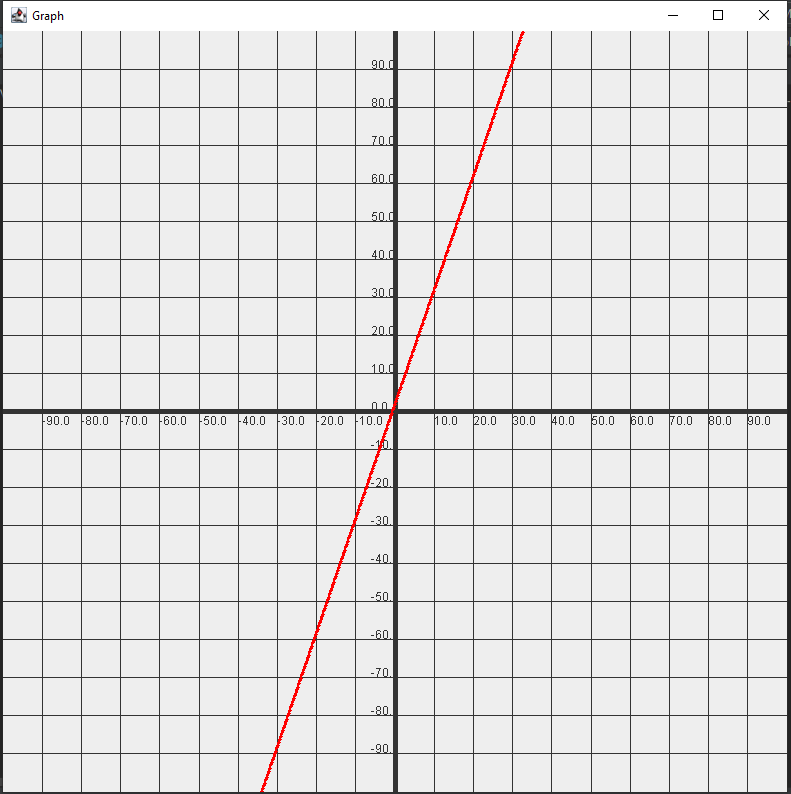
\includegraphics[width=3cm, height=3cm]{graph3x+2.PNG}        &  P   \\
2                            & plot(x\textasciicircum{}2);                                                                                           & \begin{tabular}[c]{@{}c@{}}A graph displaying\\ the function x\textasciicircum{}2 \\ should appear\end{tabular}              &    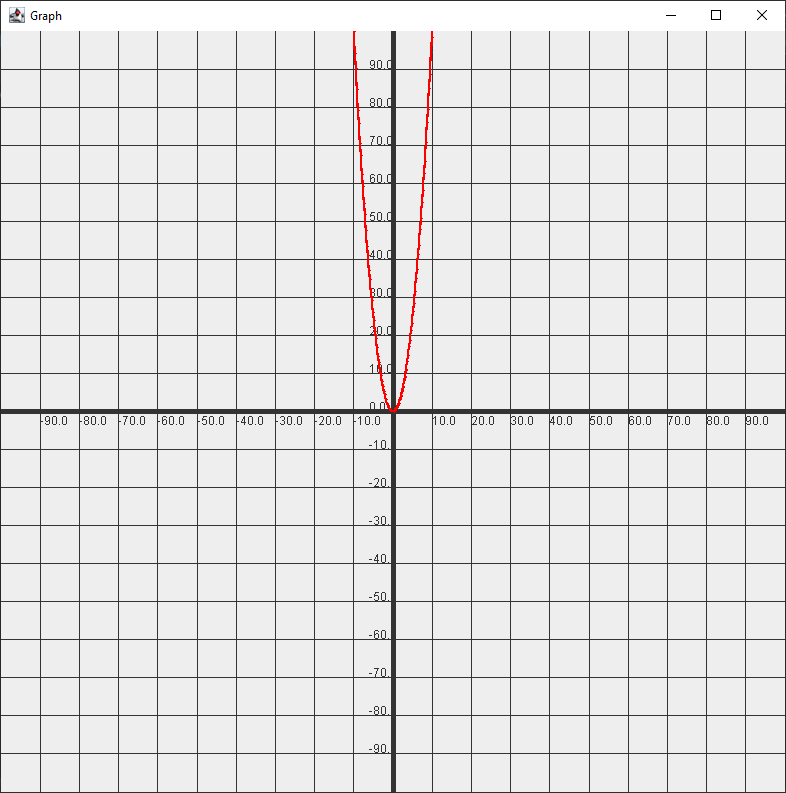
\includegraphics[width=3cm, height=3cm]{graphx2.PNG}      &    P \\
3                            & plot(x\textasciicircum{}3+x\textasciicircum{}2+x);                                                                    & \begin{tabular}[c]{@{}c@{}}A graph displaying\\ the correct \\ polynomial should\\ appear\end{tabular}                       & 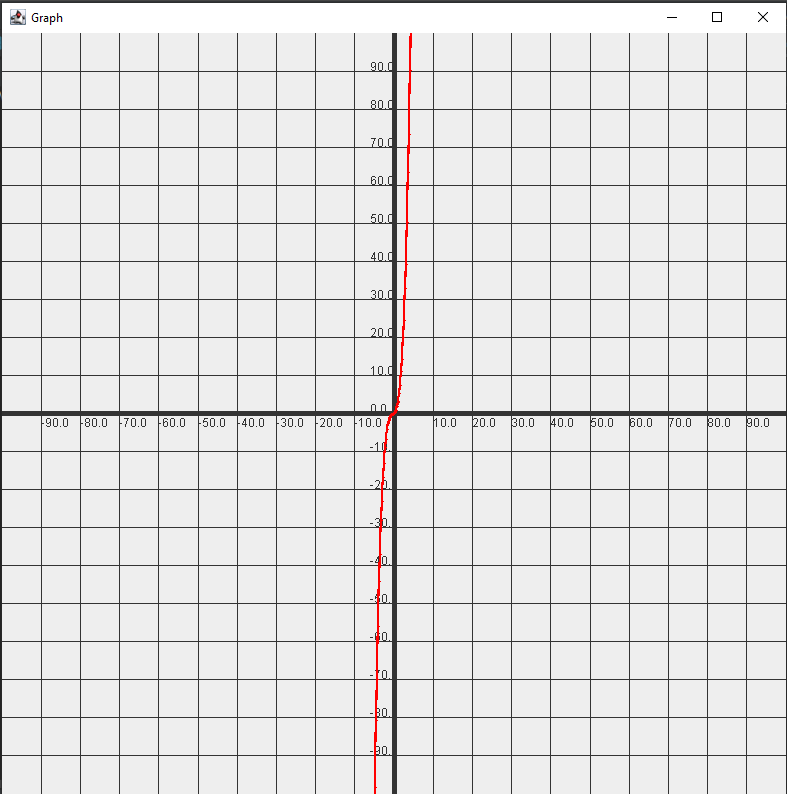
\includegraphics[width=3cm, height=3cm]{graphpolynomial.PNG}         &  P   \\
4                            & \begin{tabular}[c]{@{}l@{}}minPoint(-10,-1.5);\\ maxPoint(10,1.5);\\ setIncrement(1,0.5);\\ plot(sin(x));\end{tabular} & \begin{tabular}[c]{@{}c@{}}A graph displaying\\ the function sin(x)\\ should appear\end{tabular}                             &    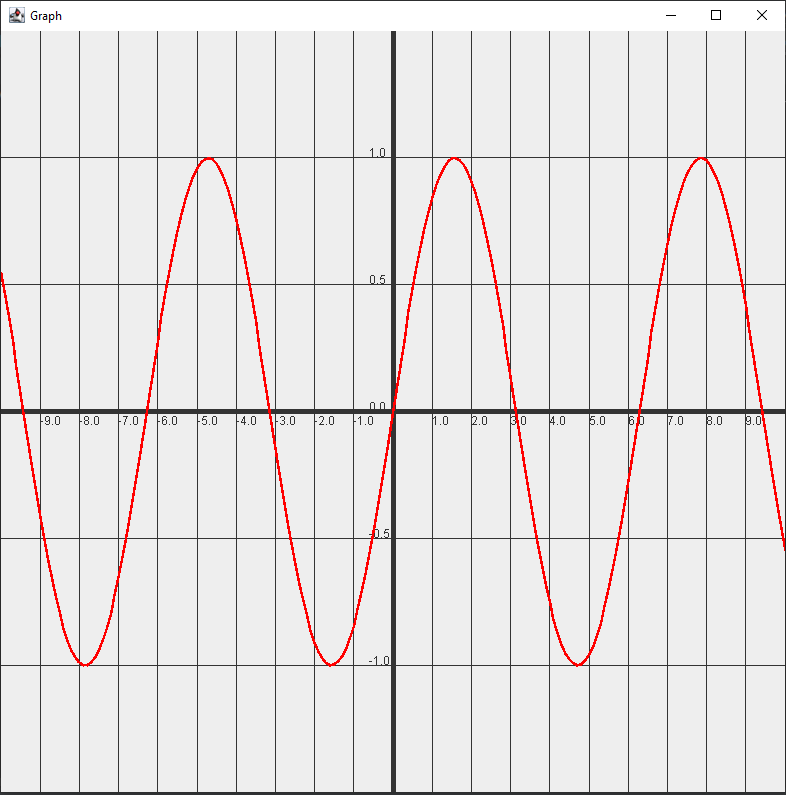
\includegraphics[width=3cm, height=3cm]{graphsinx.PNG}      &   P  \\
3                            & \begin{tabular}[c]{@{}l@{}}maxPoint(5,2);\\ minPoint(-3,-1);\\ setIncrement(1,0.2);\\plot(sin(x));\end{tabular}                       & \begin{tabular}[c]{@{}c@{}}A graph with the new\\ parameters should \\ appear displaying\\ the sin(x)\\ function\end{tabular} &    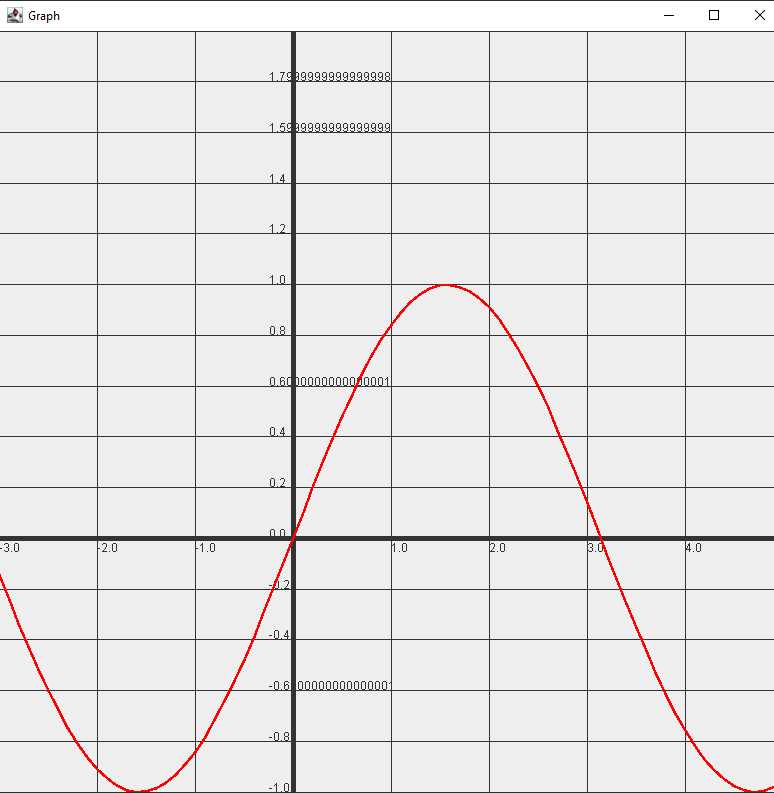
\includegraphics[width=3cm, height=3cm]{graphsinx2.PNG}      &    P
\end{tabular}
\end{table}

\begin{table}
\label{tab:req9}
\begin{tabular}{cllll}
\hline
\multicolumn{2}{l}{Requirement 9:}                 & \multicolumn{3}{l}{Simple Trig Functions}          \\ \hline
\multicolumn{2}{l}{Sub Requirement 1:}             & \multicolumn{3}{l}{Sin}                            \\
\multicolumn{1}{l}{Test No.} & Data                & Expected Outcome                   & Outcome & P/F \\
1                            & print(sin(30));     & \multicolumn{1}{c}{-0.98803162409} & -0.98803162409..        &  P   \\
2                            & print(sin(50.6));   & \multicolumn{1}{c}{0.32831349385}  &  0.32831349385..        &  P   \\
3                            & print(sin(-15));    & \multicolumn{1}{c}{-0.65028784015} & -0.65028784015..        &   P  \\
\multicolumn{2}{l}{Sub Requirement 2:}             & \multicolumn{3}{l}{Cos}                            \\
\multicolumn{1}{l}{Test No.} & Data                & Expected Outcome                   & Outcome & P/F \\
1                            & print(cos(60));     & \multicolumn{1}{c}{-0.95241298041} & -0.95241298041..        &  P   \\
2                            & print(cos(13.2));   & \multicolumn{1}{c}{0.80588395764}  &  0.80588395764..        &  P   \\
3                            & print(cos(-20));    & \multicolumn{1}{c}{0.40808206181}  &  0.40808206181..       &  P   \\
\multicolumn{2}{l}{Sub Requirement 3:}             & \multicolumn{3}{l}{Tan}                            \\
\multicolumn{1}{l}{Test No.} & Data                & Expected Outcome                   & Outcome & P/F \\
1                            & print(tan(90));     & \multicolumn{1}{c}{-1.99520041221} & -1.99520041221..        &  P   \\
2                            & print(tan(4.2));    & \multicolumn{1}{c}{1.77777977451}  &  1.77777977451..       &   P  \\
3                            & print(tan(-10));    & \multicolumn{1}{c}{-0.64836082745} & -0.64836082745..        &   P  \\
\multicolumn{2}{l}{Sub Requirement 4:}             & \multicolumn{3}{l}{Arcsin}                         \\
\multicolumn{1}{l}{Test No.} & Data                & Expected Outcome                   & Outcome & P/F \\
1                            & print(arcsin(1));   & \multicolumn{1}{c}{1.57079632679}  &  1.57079632679..        &   P  \\
2                            & print(arcsin(0.5)); & \multicolumn{1}{c}{0.52359877559}  &  0.52359877559..       &  P   \\
3                            & print(acrsin(-1));  & \multicolumn{1}{c}{-1.57079632679} & -1.57079632679..        &  P   \\
\multicolumn{2}{l}{Sub Requirement 5:}             & \multicolumn{3}{l}{Arccos}                         \\
\multicolumn{1}{l}{Test No.} & Data                & Expected Outcome                   & Outcome & P/F \\
1                            & print(arccos(1));   & \multicolumn{1}{c}{0}              &    0     & P    \\
2                            & print(arccos(0.5)); & 1.0471975512                       &  1.0471975512..        &   P  \\
3                            & print(arccos(-1));  & 3.1415926535                       &  3.1415926535..       &  P   \\
\multicolumn{2}{l}{Sub Requirement 6:}             & \multicolumn{3}{l}{Arctan}                         \\
\multicolumn{1}{l}{Test No.} & Data                & Expected Outcome                   & Outcome & P/F \\
1                            & print(arctan(1));   & 0.73539816339                      &  0.73539816339..       &  P   \\
2                            & print(arctan(0.5)); & 0.463647609                        &  0.463647609       &   P  \\
3                            & print(arctan(-1));  & -0.73539816339                     & -0.73539816339..        &    P
\end{tabular}
\end{table}

\clearpage
\section{A.3: Evidence for Tests}
\newpage
\begin{figure}
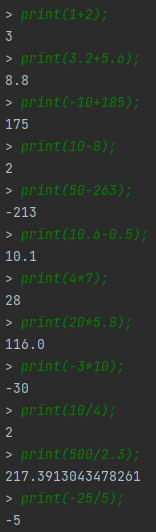
\includegraphics{Requirement 1.PNG}
\caption{Evidence for Requirement 1 testing}
\end{figure}

\begin{figure}
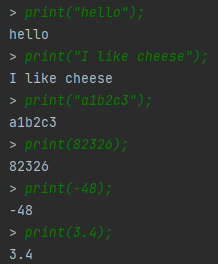
\includegraphics{Requirement 2.PNG}
\caption{Evidence for Requirement 2 testing}
\end{figure}

\begin{figure}
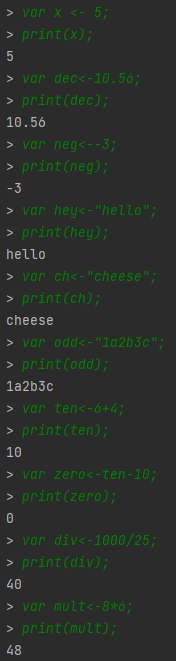
\includegraphics{Requirement 5.PNG}
\caption{Evidence for Requirement 5 testing}
\end{figure}

\begin{figure}
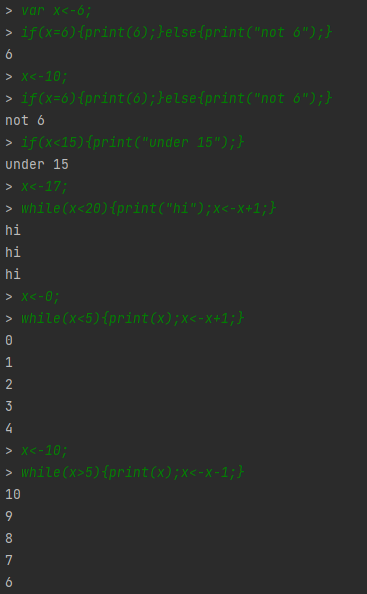
\includegraphics{Requirement 6.PNG}
\caption{Evidence for Requirement 6 testing}
\end{figure}

\begin{figure}
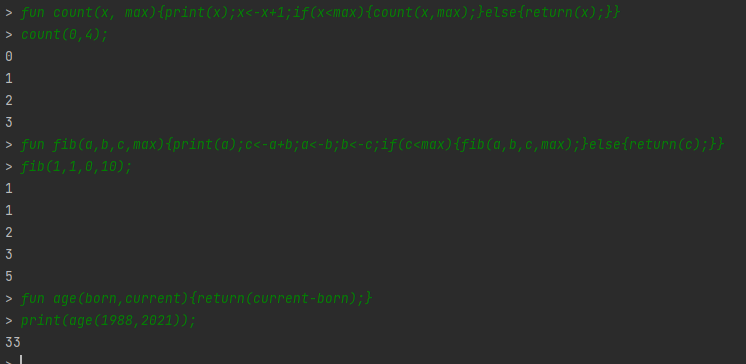
\includegraphics[width=13cm]{Requirement 7.PNG}
\caption{Evidence for Requirement 7 testing}
\end{figure}

\begin{figure}
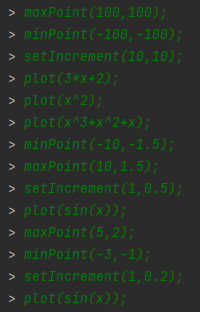
\includegraphics{Requirement 8.PNG}
\caption{Evidence for Requirement 8 testing}
\end{figure}

\begin{figure}
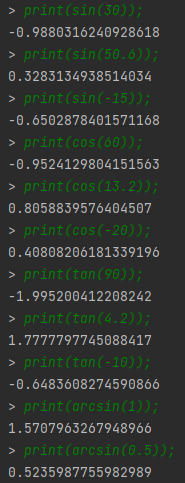
\includegraphics{Requirement 9A.PNG}
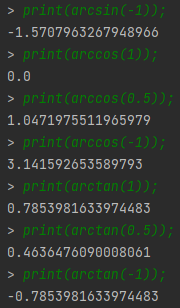
\includegraphics{Requirement 9B.PNG}
\caption{Evidence for Requirement 9 testing}
\end{figure}

\end{document}

